\chapter{Advanced Control}\indexmain{advanced control}\label{cha:transaction}

In this chapter we'll have a look at advanced graph rewrite sequence constructs,
with the \indexed{subsequences} and the backtracking double angles as the central statements.


%%%%%%%%%%%%%%%%%%%%%%%%%%%%%%%%%%%%%%%%%%%%%%%%%%%%%%%%%%%%%%%%%%%%%%%%%%%%%%%%%%%%%%%%%%%%%%%%
\section{Sequence Definitions (Procedural Abstraction )} \label{sec:sequencedefinition}
\begin{rail}
  RewriteSequenceDefinition: 
    ('def' | 'sequence') RewriteSequenceSignature lbrace RewriteSequence rbrace;
  RewriteSequenceSignature: 
    SequenceName ('(' ((InVariable ':' Type)*',') ')')? \\ (':' '(' ((OutVariable ':' Type)*',') ')')?
	;
\end{rail}\ixnterm{RewriteSequenceDefinition}\ixnterm{RewriteSequenceSignature}

If you want to use a sequence or sequence part at several locations, just factor it out into a \indexed{sequence definition} and reuse with its name as if it were a rule.
A sequence definition declares input and output variables; 
when the sequence gets called the input variables are bound to the values it was called with.
If and only if the sequences succeeds, the values from the output variables get assigned to the assignment target of the sequence call.
Thus a \indexed{sequence call} behaves as a rule call, cf. \ref{sec:ruleapplication}.

A sequence definition may call itself recursively, as can be seen in example \ref{ex:recseq}.

The compiled sequences must start with the \texttt{sequence} keyword in the rule file.
The interpreted sequences in the shell must start with the \texttt{def} keyword; a shell sequences can be overwritten with another shell sequence in case the signature is identical. (Overwriting is needed in the shell to define direct or mutually recursive sequences as a sequence must be defined before it can get used; apart from that it allows for a more rapid-prototyping like style of development in the shell.)

\begin{example}
\label{ex:recseq}
\begin{grgen}
def rec(depth:int) {\
  if{ {depth<::MAXDEPTH}; foo() ;> rec(depth+1); bar() }\
}
\end{grgen}
This example shows a sequence defined in the shell which is executing itself recursively.
The host graph is transformed by applying \texttt{MAXDEPTH} times the rule \texttt{foo}, until finally the rule \texttt{bar} is executed. The result of the sequence is the result of \texttt{bar}, returned back from recursion step to recursion step while unwinding the sequence call stack. 
\end{example}


%%%%%%%%%%%%%%%%%%%%%%%%%%%%%%%%%%%%%%%%%%%%%%%%%%%%%%%%%%%%%%%%%%%%%%%%%%%%%%%%%%%%%%%%%%%%%%%%
\section{Transactions, Backtracking, and Pause Insertions}\label{sec:extctrl}

The extended control constructs offer further rule application control in the form of \indexed{transaction}s, \indexed{backtracking}, and \indexed{pause insertions}.

\begin{rail} 
  ExtendedControl: 
    '<' RewriteSequence '>' | 
    '<<' RuleExecution ';;' RewriteSequence '>>' |
    '/' RewriteSequence '/'
	;
\end{rail}

Graph rewrite sequences can be processed \indexed{transaction}ally by using angle brackets (\texttt{<>}), i.e.
if the return value of the nested sequence is \texttt{false}, all the changes carried out on the host graph will be rolled back.
Nested transactions\indexmainsee{nested transaction}{transaction} are supported, i.e. a transaction which was committed is rolled back again if an enclosing transaction fails.

Transactions as such are only helpful in a limited number of cases, but they are a key ingredient for backtracking, which is syntactically specified by double angle brackets (\texttt{<<r;;s>>}.
The semantics of the construct are:
First compute all matches for rule \texttt{r}, then start a transaction.
For each match: execute the rewrite of the match, then execute \texttt{s}.
If \texttt{s} failed then rollback and continue with the loop.
If \texttt{s} succeeded then commit and break from the loop.
On first sight this may not look very impressive, but this construct in combination with recursive sequences is the key operation for crawling through \indexed{search space}s or for the unfolding of \indexed{state space}s.

The backtracking double angles separate matching from rewriting: first all matches are found, but then only one after the other is applied, without interference of the other matches.
The ``without interference of other matches'' statement is ensured by rolling back the changes of the application of the previous match, and much more, of the entire sequence which followed the rewriting of the previous match.

If you are just interested in the first goal state stumbled upon which satisfies your requirements during a search,
then you only need to give a condition as last statement of the sequence which returns true if the goal was reached; the iteration stops exactly in the target state.
When you are interested in finding all states which satisfy your requirements, or even in enumerating each and every state, just force backtracking by noting down the constant false as last element of the sequence.

The backtracking construct encodes a single decision point of a search, splitting into breadth along the different choices available at that point, and further continuing the search in the sequence.
When this point of splitting into breadth is contained in a sequence,
and this sequence calls itself again recursively on each branch of the descision taken,
you get a recursion which is able to search into depth,
continuing decision making on the resulting graph of the previous decision. 

\begin{figure}[htbp]
  \centering
  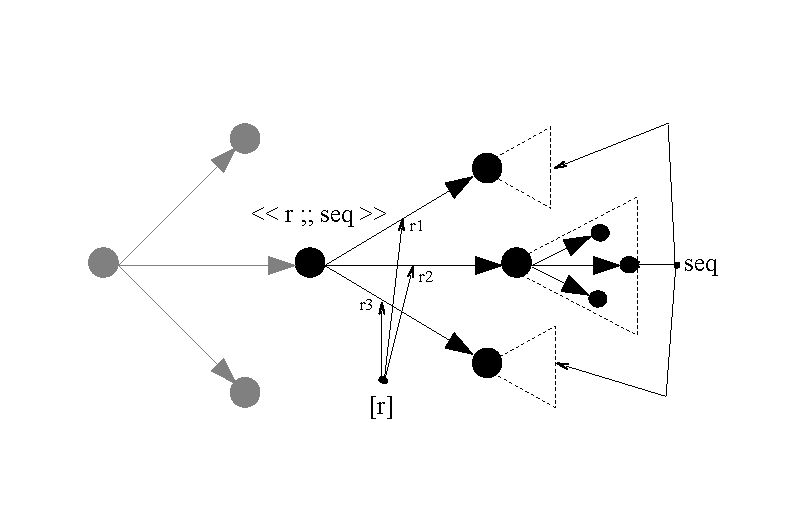
\includegraphics[width=\textwidth]{fig/SearchSpace}
  \caption{Search space illustration, a bullet stands for a graph}
  \label{figsearchspace}
\end{figure}

With each sequence call advancing one step into depth and each backtracking angle advancing into breadth, you receive a depth-first enumeration of an entire search space (as sketched in \ref{figsearchspace}).
Each state is visited in \emph{temporal succession}, with only the most recent state being available in the graph.
But maybe you want to keep each state visited, because you are interested in viewing all results at once, or because you want to compare the different states.
As there is only one host graph in \GrG, keeping each visited state requires a partition of the host graph into separate subgraphs, each denoting a state.

After you changed the modeling from a host graph to a state space graph consisting of multiple subgraphs, each representing one of the graphs you normally work with, 
you can materialize the search space visited in temporal succession into a state space graph,
by copying the subgraphs (which are normally only existing at one point in time) during \indexed{pause insertion}s out into space.
When subgraphs would be copied without pause insertions, they would be rolled back during backtracking; but effects applied on the graph from \texttt{/ in between here /} are bypassing the recording of the transaction undo log and thus stay in the graph, even if the transaction fails and is rolled back. 

When you have switched from a depth-first search over one single current graph to the unfolding of a state space graph containing all the subgraphs reached, you may compare each subgraph which gets enumerated with all the already available subgraphs, and if the new subgraph already exists (i.e. is isomorph to another already generated subgraph), you may refrain from inserting it.
This \indexed{symmetry reduction} allows to save the space and time needed for storing and computing equivalent branches otherwise generated from the equivalent states. 
But please note that the \texttt{==} operator on graphs is optimized for returning early when the graphs are different; when the graphs are isomorphic you have to pay the full price of graph isomorphy checking.
This will happen steadily with \indexed{automorphic pattern}s and then degrade performance.
To counter this filter the matches which cover the same spot in different ways, see \ref{sub:extflt} on how to do this.
Merging states with already computed ones yields a DAG-formed state space, instead of the always tree like search space.
Have a look at the transformation techniques chapter for more on state space enumeration \ref{sec:statespaceenum} and copying \ref{subsub:copystructure}.
One caveat of the transactions and backtracking must be mentioned: rollback might lead to an incorrect graph visualization when employed from the debugger.
This holds especially when using grouping nodes to visualize subgraph containment (\ref{sub:visual}). You must be aware that you can't rely on the online display as much as you can normally, and that you maybe need to fall back to an offline display by opening a \texttt{.vcg}-dump of the graph written in a situation when the online graph looked suspicious; a dump can be written easily in a situation of doubt from the debugger pressing the \texttt{p} key. 

\begin{note}
While a transaction or a backtrack is pending, all changes to the graph are recorded into some kind of undo log, which is used to reverse the effects on the graph in the case of rollback (and is thrown away when the nesting root gets committed).
So these constructs are not horribly inefficient, but they do have their price --- if you need them, use them, but evaluate first if you really do.
\end{note}


%%%%%%%%%%%%%%%%%%%%%%%%%%%%%%%%%%%%%%%%%%%%%%%%%%%%%%%%%%%%%%%%%%%%%%%%%%%%%%%%%%%%%%%%%%%%%%%%
\section{For Loops and Indeterministic Choice}

\begin{rail}
  ExtendedControl:
    'for' lbrace Variable ':' Type\\
    (';' |
    'in' Function '(' Parameters ')' ';' |
    'in' '[' '?' r ']' ';')\\
    RewriteSequence rbrace
    ;
\end{rail}\ixkeyw{for}\label{forgraphelem}\label{forincidentadjacent}\label{formatch}

The \texttt{for} loop without containment is iterating over all the elements in the current host graph which are compatible to the type given.
The iteration variable is bound to the currently enumerated graph element, then the sequence in the body is executed.
The type of the iteration variable must be statically known to be of a node or edge type.

If you iterate a node type from a graph, you may be interested in iterating its incident edges or its adjacent nodes.
This can be achieved with a for neighbouring elements loop, which binds the iteration variable to an edge in case the \emph{Function} is one of \texttt{incoming}, \texttt{outgoing}, or \texttt{incident}. 
Or which binds the iteration variable to a node in case the \emph{Function} is one of \texttt{adjacentIncoming}, \texttt{adjacentOutgoing}, or \texttt{adjacent}.
The admissible \emph{Parameters} are the source node, or the source node plus the incident edge type, or the source node plus the incident edge type, plus the adjacent node type ---
that's the same as for the sequence expression functions explained in \ref{neighbouringelementsfunctions}/Connectedness queries.
In contrast to these set returning functions, this loop contained functions enumerate nodes/edges multiple times in case of reflexive or multi edges.

The third \texttt{for} loop introduced here, the for matches loop, allows to iterate through the matches found for an all-bracketed rule reduced to a test; i.e. the rule is not applied, we only iterate its matches.
The loop variable must be of a statically known \texttt{match<r>} type with \texttt{r} being the name of the rule matched.
The elements (esp. the nodes and edges) of the pattern of the matched rule can then be accessed by applying the \texttt{.}-operator on the loop variable, giving the name of the element of interest after the dot.
Note: the elements must be assigned to a variable in order to access their attributes, a direct attribute access after the match access is not possible.
Note: the match object allows only to access the top level nodes, edges, or variables.
If you use subpatterns or nested patterns and want to access elements found by them, you have to \texttt{yield}(\ref{sub:yield}) them out to the top-level pattern.

The most important \texttt{for} loop, the one iterating a container, for enumerating the elements contained in storages, was already introduced here: \ref{forstorage}.
All \texttt{for} loops fail if one of the sequence executions failed, and succeed otherwise.

\begin{rail}
  ExtendedControl:
		'highlight' '(' Arguments ')'
    ;
\end{rail}\ixkeyw{highlight}
The \texttt{highlight} sequence highlights the arguments given as a quoted text in the graph;
it does what the \texttt{(h)ighlight} command does in the debugger, see \ref{highlight}, just programmed from the sequences. 
Arguments is a comma-separated list of variable names or visited flag ids, the graph elements contained in the variables are highlighted, as are the graph elements marked by the visited flag.

\begin{rail} 
  ExtendedControl: 
	dollar (percent)? (ampersand | '|' | doubleampersand | '||') '(' SequencesList ')' |
	dollar (percent)? '.' '(' WeightedSequencesList ')' |
	(dollar (percent)? )? lbrace '<' ((RuleExecution)+(',')) '>' rbrace
	;
  SequencesList:
	RewriteSequence ((',' RewriteSequence)*())
	;
  WeightedSequencesList:
	WeightedSequence ((',' WeightedSequence)*())
	;
  WeightedSequence:
	FloatingNumber RewriteSequence
	;
\end{rail}\ixnterm{SequencesList}

The \indexed{indeterministic choice} operators execute chosen elements from a sets of rules or sequences.
The \indexed{random-all-of operators} given in function call notation with the dollar sign plus operator symbol as name have the following semantics:
The strict operators \verb/|/ and \verb/&/ evaluate all their subsequences in random order returning the disjunction resp. conjunction of their truth values.
The lazy operators \verb/||/ and \verb/&&/ evaluate the subsequences in random order as long as the outcome is not fixed or every subsequence was executed 
(which holds for the disjunction as long as there was no succeeding rule and for the conjunction as long as there was no failing rule).
A \indexed{choice point} may be used to define the subsequence to be executed next.

The \indexed{some-of-set braces} \verb/{(r,[s],$[t])}/ matches all contained rules and then executes the ones which matched.
The \indexed{one-of-set braces} \verb/${(r,[s],$[t])}/ (some-of-set with random choice applied) matches all contained rules and then executes at random one of the rules which matched
(i.e. the one match of a rule, all matches of an all bracketed rule, or one randomly chosen match of an all bracketed rule with random choice).
The one/some-of-set is true if at least one rule matched and false if no contained rule matched.
A \indexed{choice point} may be used on the one-of-set; it allows you to inspect the matches available graphically before deciding on the one to apply. 

The \indexed{weighted one operator} \verb/$.(w1 s1, ..., wn sn)/ is executed like this:
the weights \texttt{w1-wn} (numbers of type double) are added into a series of intervals,
then a random number (uniform distribution) is drawn in between \texttt{0.0} and \texttt{w1+...+wn},
the subsequence of the interval the number falls into is executed,
the result of the sequence is the result of the chosen subsequence.


%%%%%%%%%%%%%%%%%%%%%%%%%%%%%%%%%%%%%%%%%%%%%%%%%%%%%%%%%%%%%%%%%%%%%%%%%%%%%%%%%%%%%%%%%%%%%%%%
\section{Quick Reference Table}

Table~\ref{seqtab} lists most of the operations of the graph rewrite sequences at a glance.

%\makeatletter
\begin{table}[htbp]
\begin{minipage}{\linewidth} \renewcommand{\footnoterule}{} 
\begin{tabularx}{\linewidth}{|lX|}
\hline
\texttt{(w)=s(w)} & Calls a sequence \texttt{s} handing in \texttt{w} as input and writing its output to \texttt{w}; defined e.g. with \texttt{sequence s(u:Node):(v:Node)} \texttt{\{ v=u \}}.\\
\hline
\texttt{<s>}	& Execute \texttt{s} transactionally (rollback on failure).\\
\texttt{<<r;;s>>}	& Backtracking: try the matches of rule \texttt{r} until \texttt{s} succeeds.\\
\texttt{/ s /}	& Pause insetion: execute \texttt{s} outside of the enclosing transactions and sequences, i.e. the changes of \texttt{s} are not rolled back.\\
\hline
\texttt{highlight(vars)} & Highlights the content of the variables in the graph. \\
\hline
\texttt{\$\{<r1,[r2],\$[r3]>\}}	& Tries to match all contained rules, then rewrites indeterministically one of the rules which matched. True if at least one matched.\\
\hline
\texttt{for\{v in u; t\}}	& Execute \texttt{t} for every \texttt{v} in storage set \texttt{u}. One \texttt{t} failing pins the execution result to failure.\\
\texttt{for\{v->w in u; t\}}	& Execute \texttt{t} for every pair (\texttt{v},\texttt{w} in storage map \texttt{u}. One \texttt{t} failing pins the execution result to failure.\\
\texttt{for\{v:match<r> in [?r]; t\}}	& Execute \texttt{t} for every match \texttt{v} from rule \texttt{r}. One \texttt{t} failing pins the execution result to failure.\\
\texttt{for\{v:T; s\}}	& Execute \texttt{s} for every \texttt{v} of type \texttt{T} available in the graph. One \texttt{s} failing pins the execution result to failure.\\
\texttt{for\{v in func(w); s\}}	& Execute \texttt{s} for every edge/node incident/adjacent to \texttt{w} . One \texttt{s} failing pins the execution result to failure.\\
\hline
\texttt{\{comp\}}	& An unspecified sequence computation (see table \ref{comptab}).\\
\hline
\end{tabularx}\indexmain{\texttt{<>}}\indexmain{\texttt{<<;>>}}
\end{minipage}\\
\\ 
{\small Let \texttt{r}, \texttt{s}, \texttt{t} be sequences, \texttt{u}, \texttt{v}, \texttt{w} variable identifiers, \texttt{<op>} $\in \{\texttt{|}, \texttt{\textasciicircum}, \texttt{\&}, \texttt{||}, \texttt{\&\&}\}$ }%and \texttt{n}, \texttt{m} $\in \N_0$.}
\caption{Sequences at a glance}
\label{seqtab}
\end{table}
%\makeatother
 
% todo: beispiele im text bringen
